\documentclass[border=9pt]{standalone}
\usepackage[fontset=fandol]{ctex}
\usepackage{amsmath,amssymb,tikz}
\usetikzlibrary{arrows.meta,calc,decorations.pathmorphing}
\tikzset{arr/.style={-{Stealth[length=2mm]},semithick}}
\begin{document}

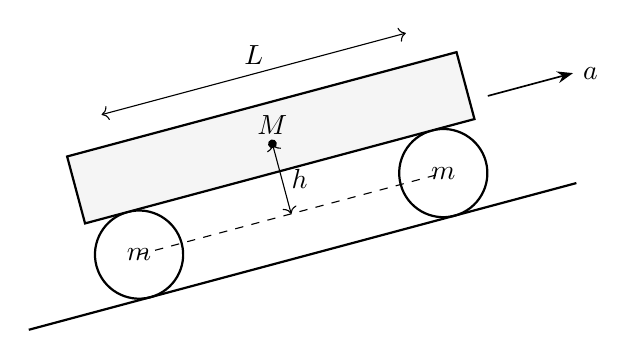
\begin{tikzpicture}[scale=.8,rotate=15]
\draw[thick] (-1,0)--(8,0);
\draw[thick] (1,.7) circle(.7);\draw[thick] (6,.7) circle(.7);
\draw[thick,fill=gray!8] (.3,1.4) rectangle(6.7,2.5);
\fill (3.5,1.85) circle(2pt) node[above] {$M$};
\draw[dashed] (1,.7)--(6,.7);
\draw[<->] (1,3)--(6,3) node[midway,above] {$L$};
\draw[<->] (3.5,.7)--(3.5,1.85) node[midway,right] {$h$};
\node at (1,.7) {$m$};\node at (6,.7) {$m$};
\draw[arr] (7,1.7)--(8.4,1.7) node[right] {$a$};
\end{tikzpicture}

\end{document}
